\chapter{Analysis}
\label{chap:analysis}
	As with so many projects, toy never start from scratch. In this chapter I will investigate exising solutions solving the same problem -- or one fairly similar to -- as desribed in chapter \ref{chap:intro}.

	\section{Existing Available Tools}
		Having reseached which tools are currently available, I've condensed my findings into the following list. 

		\begin{itemize}
			\item LastPass, and Similar Solutions
			\item KeePass, and Similar Solutions
			\item Rattic (https://rattic.org)
			\item Encryptr (https://encryptr.org/)
			\item VAULT (https://vaultproject.io/)
			\item Vault (https://www.zoho.com/vault/application-security.html)
			\item TeamPasswordManager (http://teampasswordmanager.com)
			\item Secret Server Express (http://thycotic.com/products/secret-server/express/)
			\item Simple Safe (https://www.simplesafe.net/)
			\item PassWork (https://passwork.me/)
			\item SimpleVault (http://simplevault.sourceforge.net)
			\item PasswordState (http://www.clickstudios.com.au/)
		\end{itemize}

		\subsection{LastPass, and Similar Solutions}
		\label{subsec:lastpass}
			In the name of usability services such as LastPass\footnote{https://lastpass.com/}, PassPack\footnote{https://www.passpack.com/}, DashLane\footnote{https://www.dashlane.com/}, and so many others grew popular, and it is easy to understand why. Enabling you to access your passwords from several devices, through native apps or the browser, it seemed like it was the perfect match of usability and security. To not repeat myself over and over again, I will focus on LastPass \emph{(due to them being the most well-known)} as a representation of this group.

			If we start by looking at the technical details of LastPass, they quote themselves using 256-bit AES encryption, and applies PBKDF2, in order to make it as difficult as possible, to crack stored data. For maximum security, both encryption and decryption, is done client side\cite{lastpass_cleintsideencryption}, as to avoid transferring the actual password, unencrypted, to their servers. Encryption and decryption is done using the master password, which is never actually sent to their servers. Finally, as is to be expected, all connections to LastPass' servers, are SSL encrypted.

			Having examined the technical aspect, we need to pay attention to the usability as well. Looking at their web UI, it shows a reasonably straight forward design. Allowing the user to organise passwords folders, creating a two-level structure, as seen on figure \ref{fig:lastpass_main} on page \pageref{fig:lastpass_main}. While this \emph{does} allow the user some level of organisation, several levels would have been preferable. Additionally, LastPass is renowned for their apps and plugins, covering all major operating systems and browsers, creating a near seamless integration, when it comes to addition of new passwords and auto-filling stored passwords.

			However, with the recent leak from LastPass \cite{lastpass_leak}, more and more users grew suspicious of these services. No matter how much encryption you apply, you can not get around the fact, that you have to \emph{trust} LastPass to both be completely honest about their encryption technology, \emph{and} storing your sensitive data. In many of the more sceptical user's eyes, this is a huge drawback, and why this solution is deemed unusable to solve the problem at hand.

			\begin{figure}[h!]
				\centering
				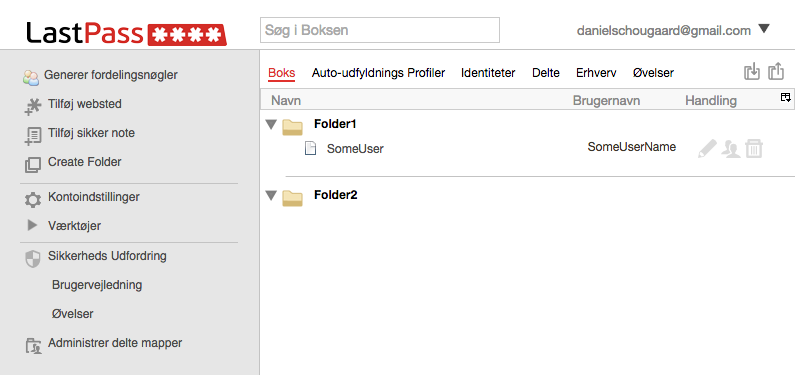
\includegraphics[width=\textwidth]{figures/analysis/lastpass_main.png}
				\caption{Screenshot of LastPass' main view, in a browser.}
				\label{fig:lastpass_main}
			\end{figure}



		\subsection{KeePass}
			As the users grew suspicious of LastPass and the likes, a lot of them moved over to e.g. KeePass\footnote{https://keepass.org}, which allows the user to store the passwords in a local file. While there exists a plethora of tools similar to KeePass, I will focus on KeePass as the representative of the bunch, much as in section \ref{subsec:lastpass}.

			If we again start by examining the technical details, as of version 2.x KeePass only -- per default -- offers AES-256 encryption, which is seen on figure \ref{fig:keepass_create_security} on page \pageref{fig:keepass_create_security}, with additional algorithm choices available through plugins \cite{keepass_security}. This enables users to tailor the encryption security, to their own needs -- and beliefs. 

			Looking at the main UI, of which an example is shown on figure \ref{fig:keepass_main} on page \pageref{fig:keepass_main}, KeePass features exactly that which could be improved in LastPass: A tree like structure, in order to completely organise passwords. Other than that, there isn't anything noteworthy to say about their UI: It features the necessary and that's about it. A final thing worth mentioning, is that their password generator is completely customisable, as seen on figure \ref{fig:keepass_newpassword_passwordgen} on page \pageref{fig:keepass_newpassword_passwordgen}. You can manually choose, exactly which character sets, you wish to be in your passwords, enabling you to have passwords using local accents should the target system support it, which is a really nifty feature.

			However, having praised the features of KeePass, it does lack something extremely important: Usability. More precisely, it lacks distribution. Since KeePass works on a local file, it would only inherently work on a \emph{single} device. Should one wish to distribute it, another tool has to be involved. File synchronisation tools, such as Dropbox, Google Drive, or Syncthing could be used, in order to create a distributed-ish feel to KeePass. However, you do still rely on a third party tool, which is a drawback. Additionally, there is the lack of cross-platform compatibility, since \emph{officially} KeePass only supports Windows. Granted, there exists unofficial ports for Linux, OS X, Android, etc., but you have to trust the developers of these unofficial applications. By extension, this introduces the threat of security breaches, which renders it as a less than ideal setup.

			\begin{figure}[h!]
				\centering
				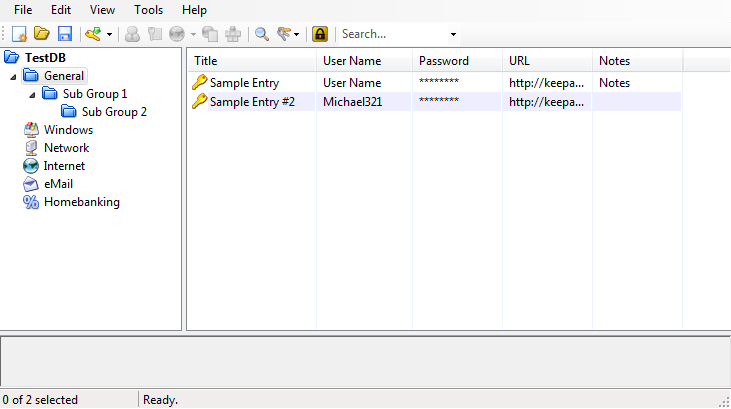
\includegraphics[width=\textwidth]{figures/analysis/keepass_mainview.png}
				\caption{Screenshot of KeePass' main view.}
				\label{fig:keepass_main}
			\end{figure}

			\begin{figure}[h!]
				\centering
				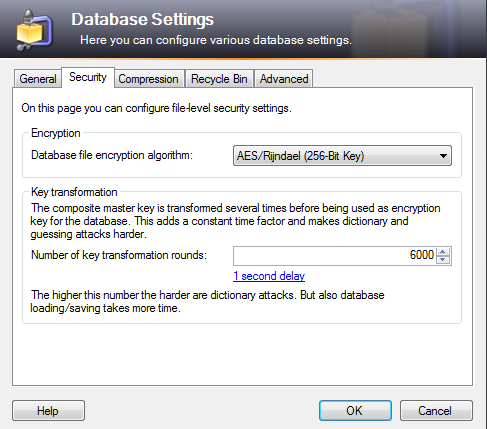
\includegraphics[width=0.7\textwidth]{figures/analysis/keepass_create_security.png}
				\caption{Screenshot of KeePass' security options.}
				\label{fig:keepass_create_security}
			\end{figure}
		
			%\begin{figure}[h!]
			%	\centering
			%	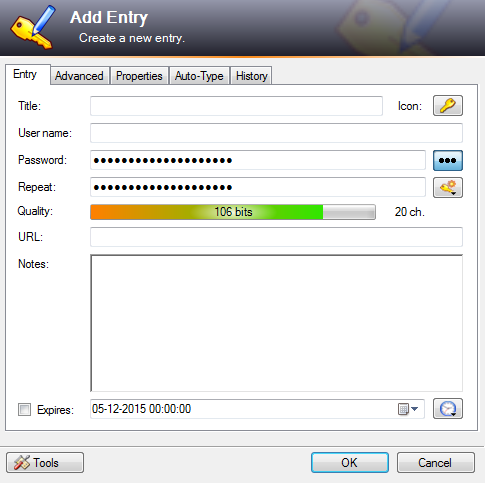
\includegraphics[width=\textwidth]{figures/analysis/keepass_newpassword_main.png}
			%	\caption{.}
			%	\label{fig:}
			%\end{figure}

			\begin{figure}[h!]
				\centering
				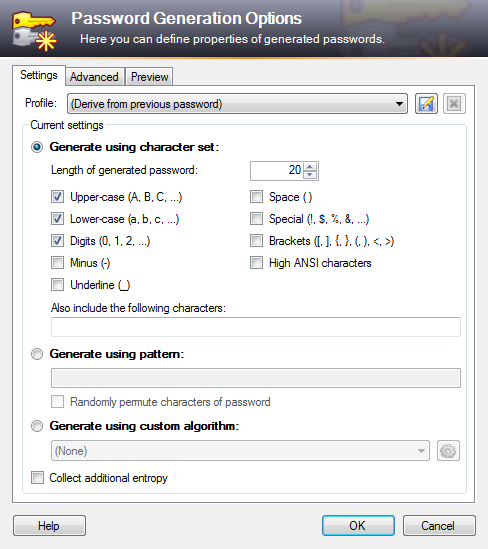
\includegraphics[width=0.7\textwidth]{figures/analysis/keepass_newpassword_passwordgen.png}
				\caption{Screenshot of KeePass' password generator settings.}
				\label{fig:keepass_newpassword_passwordgen}
			\end{figure}

		\subsection{Rattic}
			Rattic\cite{rattic_frontpage} represents a third type of password manager, and the primary focus of this thesis: A self-hosted password manager, in the so-called private cloud. While at first glance, Rattic seems to be a solution very suited to the problem described earlier, it becomes a far more sketchy solution, upon investigating it closely. Rattic wonderfully describe their solution as:

			\begin{quote}
				\emph{RatticDB is a password management database designed for humans. We have focused on making it able to manage passwords for a team and to make that as easy as possible.}\\\cite{rattic_frontpage}
			\end{quote}

			Since Rattic \emph{is} meant for teams it has multi-user support. Rattic organises passwords and users in groups, and these groups are used for access control. A group is a collection of users, which can access the same passwords. An example of this could be \verb=DevelopmentTeam1= and \verb=DevelopmentTeam2=. Members of team one, can access their own passwords, and members of team two can access theirs, but unless specifically stated, they can not access each others. Additionally it supports tags for their passwords, allowing for even further organisation, for their users allowing quick access to similar passwords, from across different groups.

			However, the fact that Rattic markets itself at teams, rather than individual users is evident by the fact that as per default, you can not create ``private'' passwords, which only a single user can access. To achieve that, you would need to manually create a new group -- per user -- with only said user as member. While this would work, it is very much a work-around of Rattic's default behaviour, for it to work that way.

			From a user experience point of view, Rattic is a rather friendly tool. On figure \ref{fig:rattic_main} on page \pageref{fig:rattic_main}, you see a clean, minimalistic view of available passwords. Granted, this figure is from an Admin's point of view, hence he can access both the \verb=DevelopmentTeam1= and \verb=DevelopmentTeam2= groups, and consequently passwords stored under them.

			\begin{figure}[h!]
				\centering
				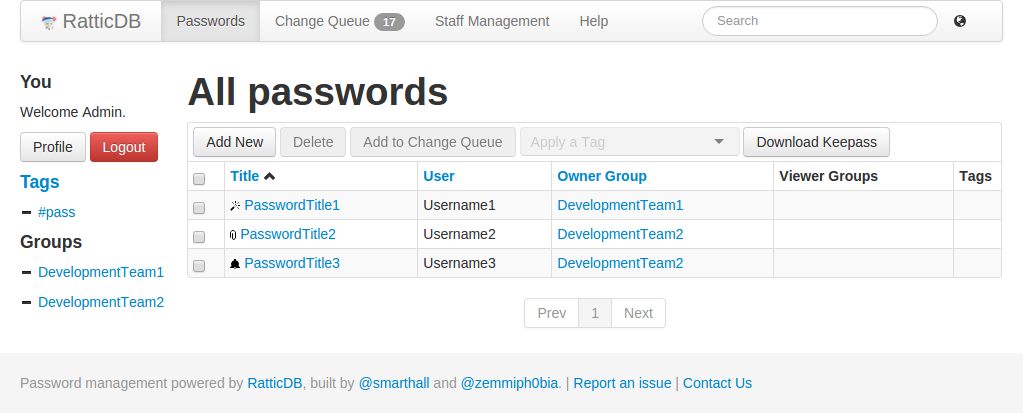
\includegraphics[width=0.95\textwidth]{figures/analysis/rattic_main.png}
				\caption{Rattic's Frontpage of their Web UI.}
				\label{fig:rattic_main}
			\end{figure}

			Adding passwords is just as easy in KeePass, cf. figure \ref{fig:rattic_newpassword_main} on page \pageref{fig:rattic_newpassword_main}. Simply type in the details, select an owner group and submit. While the password generator, cf. figure \ref{fig:rattic_newpassword_passwordgen} on page \pageref{fig:rattic_newpassword_passwordgen}, could stand to have some additional features, it is sufficient for generating strong passwords with high enough entropy. A nifty little feature, is the \verb=Download KeePass= button, which allows a user to download passwords in the KeePass format, making it available for later offline use.

			\begin{figure}[htbp]
				\centering
				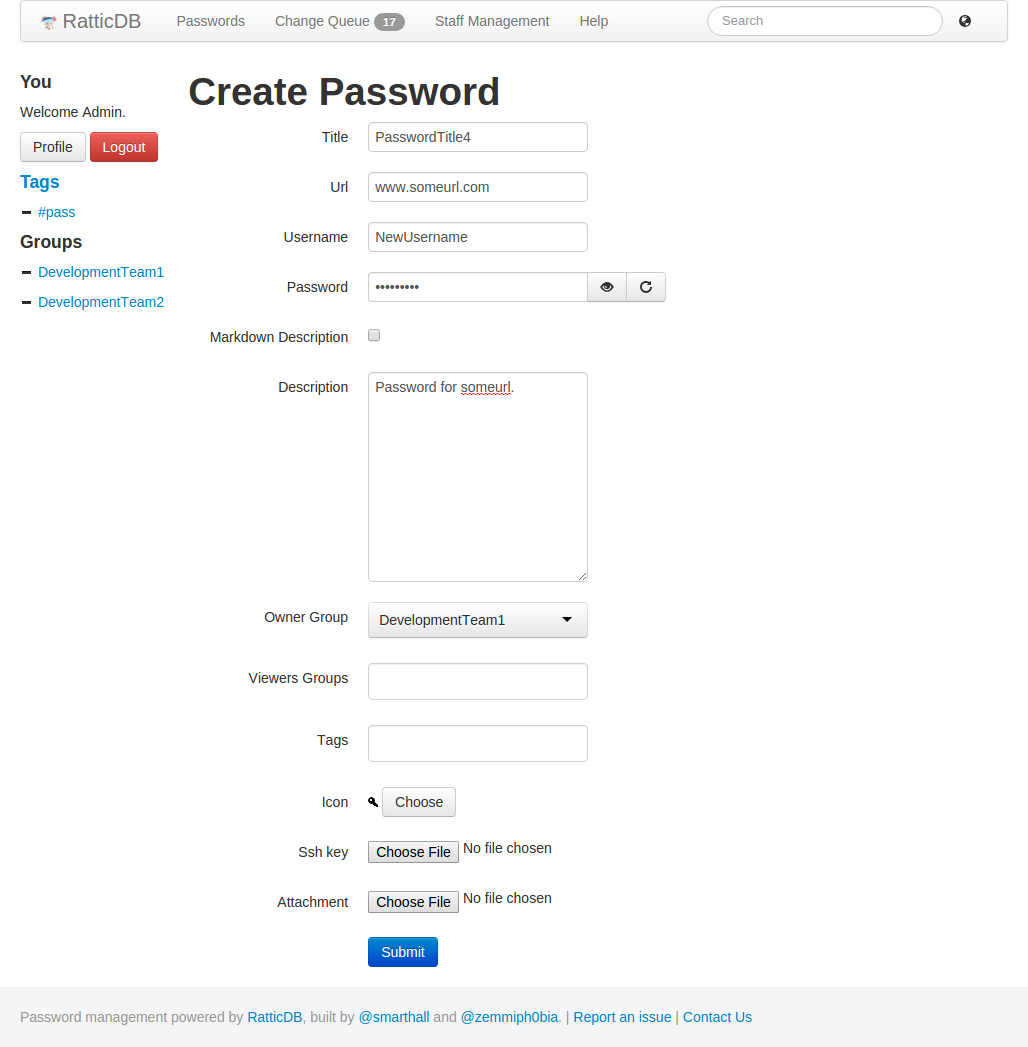
\includegraphics[width=0.95\textwidth]{figures/analysis/rattic_newpassword_main.png}
				\caption{Adding a new password, in Rattic.}
				\label{fig:rattic_newpassword_main}
			\end{figure}

			\begin{figure}[htbp]
				\centering
				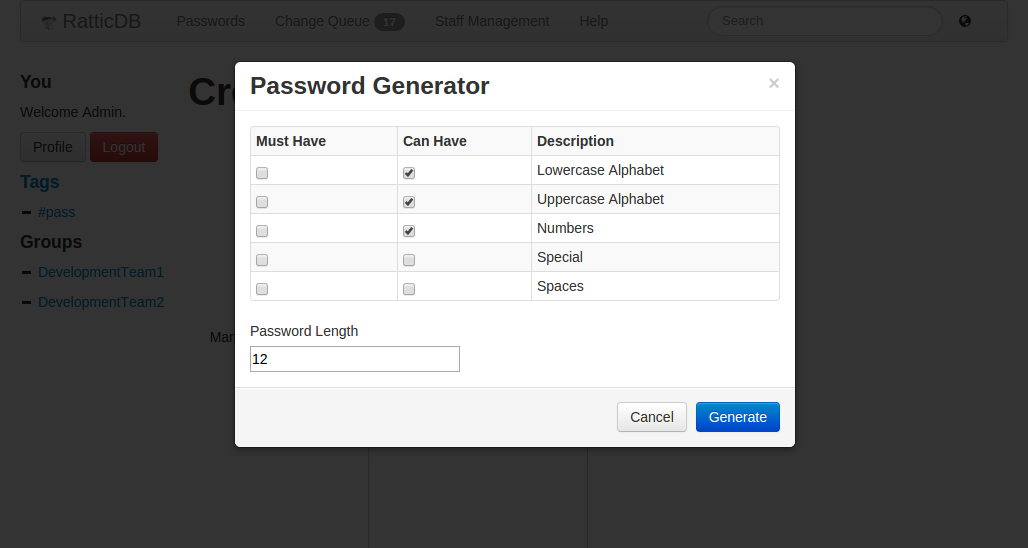
\includegraphics[width=0.95\textwidth]{figures/analysis/rattic_newpassword_passwordgen.png}
				\caption{Generating a password in Rattic.}
				\label{fig:rattic_newpassword_passwordgen}
			\end{figure}

			Having said that, there are some technical concerns, regarding Rattic. Rattic does \emph{not} encrypt passwords stored in the database -- something they are very open about. In \cite{rattic_encryption} they argue heavily for their lack of encryption, due to requiring less code and tests. They do, however, highly recommend storing the database on an encrypted drive, to ensure database protection. However, this \emph{does} mean that a sysadmin can access \emph{all} passwords, should he or she have the encryption key for the drive. Due to this, the deployment of Rattic is fairly complex, as they admit themselves. 

			Rattic is developed in Python, using the Django framework and tested on the Apache server.



		\subsection{Encryptr}
			Bordering between the type of LastPass and Rattic, Enryptr \cite{encryptr} relies on the Crypton\cite{crypton} backend\cite{encryptr_backend}, available hosted at SpiderOak\cite{crypton_spideroak}. Per default, Encryptr \emph{only} supports hosting passwords at the Crypton backend, hosted at SpiderOak. However, it \emph{is} possible to run this in the private cloud, with your own Crypton backend. \emph{But} it requires manually editing source files\cite{encryptr_selfhost}, which makes the setup a pain. So not only would you have to set up Crypton, and its requirements, you would have to download the source of the apps, change the specified line of code, compile and \emph{then} you could use it. Because of this technical aspect, usability is virtually zero, as you would need to be fairly confident behind a keyboard, to successfully set this up.

			Having said that, the UI of Encryptr is \emph{very} minimalistic and sleek, which both is a good and a bad thing. As seen on figure \ref{fig:encryptr_main} on page \pageref{fig:encryptr_main}, all passwords are stored in a \emph{single} list: There is \emph{no} organisation, other than labels. Granted, they do support searching, but somehow that still makes it very confusing, if more than a handful of passwords or secrets are stored, and since Encryptr not only supports storing passwords, but also credit card information and general secrets, this could be achieved fairly quickly.

			Adding a passwords shows something disturbing: Lack of a decent password generator, cf. figure \ref{fig:encryptr_newpassword} on page \ref{fig:encryptr_newpassword}. Once the form for adding a new password is opened, a password is generated as per some default behaviour. There is no customising entropy of the password, or even something as simple as the length.

			\begin{figure}[htbp]
				\centering
				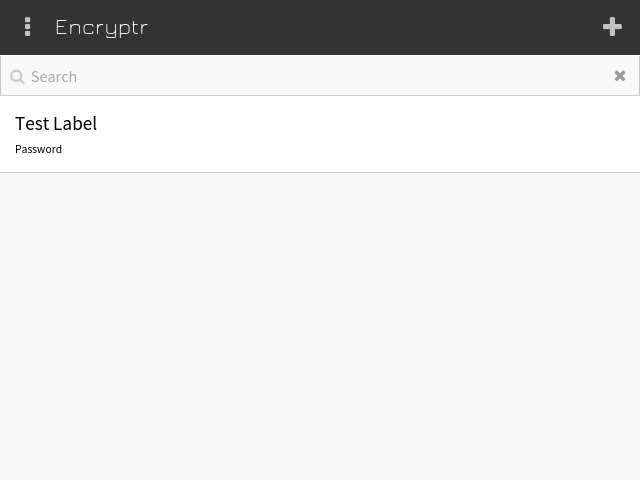
\includegraphics[width=0.95\textwidth]{figures/analysis/encryptr_main.png}
				\caption{Encryptr's main view.}
				\label{fig:encryptr_main}
			\end{figure}


			\begin{figure}[htbp]
				\centering
				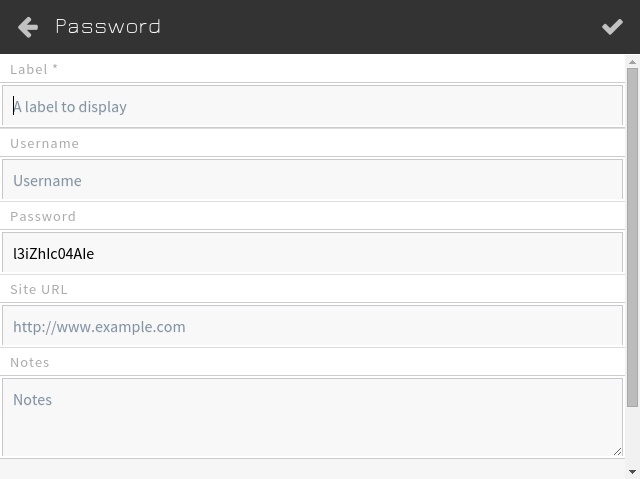
\includegraphics[width=0.95\textwidth]{figures/analysis/encryptr_newpassword_main.png}
				\caption{Adding a new password in Encryptr.}
				\label{fig:encryptr_newpassword}
			\end{figure}

			On the technical side, Crypton -- the backend -- is actually fairly interesting. Using their own definition of zero-knowledge, the developers created a complete framework for securely transferring and storing data at a remote machine\cite{crypton_paper}. They claim, that it is impossible to obtain the unencrypted data on their servers, without actually getting hold of the users private encryption key. 








		\subsection{Vault}
			ZOHO's Vault software is yet another piece of software that falls under the same category as LastPass: You upload your passwords to their servers. While they -- much like LastPass -- have a delightful UI and good user experience, it is \emph{still} hosted on a machine, someone else hosts.

			
		\subsection{VAULT (vaultproject.io)}
			Vault markets itself as a tool for ``securely accessing secrets". This tool differs greatly from the previously covered. Vault is \emph{only} a CLI / HTTP API tool. There is no graphical interface as such.

		\subsection{TeamPasswordManager}
			TeamPasswordManager aims itself at -- as the name implies -- teams, much like Rattic. This choice, is very apparent in the work flow. For instance, a password is tied to a ``project", instead of a user. Security wise, TeamPasswordManager dons some impressive features. Using the standard AES-256, with the twist of a Bcrypt approach, and two-factor authentication.

			While this software could essentially suffice, in order to meet the requirements, it would be lacking heavily in the user experience department.



		\subsection{Secret Server Express}
			Thycotic's Secret Server Express is yet another one of those pieces of software, clearly aimed at the Enterprise. Their feature list is surely impressive, but most of them are clearly aimed at larger corporations. 

			Giving no demo or screenshots of the software they're selling, it is impossible to determine the user experience of the software, however I would go as far as to wager, that it would be very focussed on enterprise workflows.

		\subsection{Simple Safe}
			Simple Safe markets itself at teams, which is not necessarily evident at a first glance. However, based on their own user experience -- and poor description -- it appears that all users have access to all passwords. This results in, that a single user can not have a private password, for their use only.

			As seen before, Simple Safe allows passwords to be organised in "groups", much like Rattic. When you switch between groups, it is very ``clonky", with a grey'ed over screen, showing it's loading -- and it takes a while. From a user experience point of view, their solution is less than optimal.

			From a encryption perspective, there isn't a lot to be told. Their rather vague description of their software, only states that they use 256 bit encryption \footnote{https://www.simplesafe.net/faqs/}, omitting their algorithm choice.


		\subsection{PassWork}
			Yet another solution, that markets itself at the enterprise, and has password data stored on a remote server. Same comments goes for this, as for LastPass, Vault (ZOHO), and Secret Server Express. 

			Their user experience seems fine, and at first glance they -- per default -- have created a private group for each user, to store private passwords in. 

		\subsection{Simple Vault}
			While Simple Vault is \emph{clearly} not aimed at enterprise use and is actually self-hosted, it does come with a bunch of downsides. First of all, it does not appear that it has the possibility for several users. Secondly, there is absolutely \emph{no} organisation: Passwords are stored single level, sorted lexicographical. Each individual password, can be protected by a passphrase, ``sort of" enabling multi-user access. However, other users will be able to see the password exists for a given website, which can be considered unfortunate.

			User experience wise, it is horrible. The design and colours are a pain to work with, the position of buttons and menus are not intuitive. Not to sound too harsh, but the design looks like it was made by a 7th grader: It does \emph{not} inspire confidence, in the developers ability to sufficiently protect my data.s

		\subsection{PasswordState}
			While PasswordState does market itself at enterprise customers, they offer a free version of their software, for teams of up to five people. Their UI is wonderful, if you are a tech geek and/or love graphs. It is very advanced since you're immediately presented with a lot of information, leading to believe it would easy scare off not-so-super-users.

			Sporting a tree level structure, PasswordState manages to create the organisation there have been lacking from the previously examined tools.

			Unfortunately, PasswordState is limited to the Windows platform, making it less than optimal for the purposes of this project. It would render it unable to be executed, from a Raspberry Pi, for instance.



		\subsection{Comparison Chart}
			\begin{table}
				\begin{tabular}{ r l l l l }
					Name 				& Encryption  & Web Accessible 		& Server Software 		& Language \& Framework 		\\
					\hline
					LastPass 			& AES-256 		& Yes			& N/A 				& N/A \\
					KeePass 			& AES-256 (more available through plugins) & No & N/A & C++ \\
					Rattic 				& None 			& Yes 			& Apache 		& Python \& Django \\
				\end{tabular}
			\end{table}



	\section{Academic Research and Tools}
	\section{Chosen Inspiration}